\chapter{Dark Matter Models}
\label{sec:theory}
\bigskip
\Contributors{Simeon Bird, Kimberly Boddy, Matthew Buckley, Francis-Yan Cyr-Racine, Will Dawson, Alex Drlica-Wagner, Juan Garc\'ia-Bellido, Maurizio Giannotti, Vera Gluscevic, Nathan Golovich, Manoj Kaplinghat, Sam McDermott, Michael Medford, Manuel Meyer, Annika Peter, Chanda Prescod-Weinstein, Oscar Straniero, Hai-Bo Yu}

In this section, we provide a brief review of several theoretical models of dark matter with a specific focus on the properties of these models that can be explored by LSST. 
We divide the domain of models into three different categories. 
We first discuss reasonably minimal extensions of the popular cold, collisionless particle dark matter paradigm (\secref{particles}). 
We then extend our discussion to much lighter axion-like particle and wave-like dark matter (\secref{axions}). 
Finally, we discuss the potential to constrain alternative compact dark matter models, with a focus on primordial black holes (\secref{machos}).
We stress that exploring a broad theoretical landscape with LSST is strongly motivated by the lack of an experimental discovery of a conventional CDM particle candidate. 

\section{Particle Dark Matter \Contact{Haibo}}
\Contributors{Haibo, Alex, Francis-Yan}
\label{sec:particles}

%\footnote{WIMPs and axions are not truly ``collisionless" because they require a coupling with other particles during their birth epoch in the early universe.  However, their interactions are so small that they are effectively collisionless particles for cosmology applications after that epoch.  Hence, WIMPs and axions are often considered to be the canonical examples of particle models for the CDM paradigm even though they are technically not completely collisionless.\AHGP{I added this.  Not sure this is the best place for it, but it would be good if this idea went somewhere.}}  

The standard \LCDM cosmological model assumes that dark matter is fully nonrelativistic and interacts purely via gravitational interactions during the process of structure formation. However, a significant dark matter thermal velocity dispersion or the presence of large non-gravitational interactions in the dark sector, such as dark matter self-interactions, couplings to other dark sector particles, or couplings to Standard Model particles, can alter the distribution of dark matter in ways that are observable with LSST. Here we focus on three representive minimal extensions to CDM -- warm dark matter (WDM), self-interacting dark matter (SIDM), and baryon-scattering dark matter (BSDM) --  to demonstrate how measurements of the distribution of dark matter can be used to constrain micro-physical particle properties of dark matter. We largely leave in-depth discussion of the particle physics responsible for producing these models to the literature; however, we do attempt to connect astrophysical observables to specific terms in the interaction Lagrangian for these models.

\subsection{Warm Dark Matter (WDM)}
\label{sec:wdm}

In the standard thermal dark matter paradigm, primordial inhomogeneities in the matter density field are washed out by collisional damping and free streaming of particle dark matter \citep{Hofmann:2001,Green:2003un, Bertschinger:2006nq, Loeb:2005pm}.  
For a canonical 100-GeV thermal relic dark matter particle \citep[\eg, the WIMP;][]{Jungman:1995df}, these processes erase cosmological perturbations with $M \leq 10^{-6} \Msun$ \citep[i.e., Earth mass;][]{Green:2003un, 2005Natur.433..389D}. 
Lighter particles continue to free stream until later times, thus suppressing the formation of structure at higher mass scales (\eg, structure formation occurs bottom-up above the free-streaming scale and top-down for scales below the free-streaming scale). Because these particles are created while they are semi-relativistic, they are conventionally referred to as warm dark matter (WDM) \citep{Bond:1983hb,Bode:2000gq,Dalcanton:2000hn}. 
WDM constitutes a subclass of sub-GeV dark matter candidates.

One well-motivated WDM candidate is a sterile neutrino, $\nu_{\rm s}$, with a mass in the keV range \citep[\eg][]{Abazajian:2017tcc,Adhikari:2017}. The most relevant Lagrangian term in this case is simply the Majorana mass term,
\begin{equation}
    \mathcal{L} \supset -\frac{1}{2}M_{\rm s}\bar{\nu}_{\rm s} \nu_{\rm s}.
\end{equation}
Interestingly, such a sterile neutrino can typically mix with active Standard Model neutrinos \citep[\eg,][]{Asaka:2005an}, allowing the former to decay and leading to a potentially observable X-ray signal \citep[\eg,]{Abazajian:2001vt}. A possible hint of such a signal has been found in deep X-ray data in the form of a narrow 3.5 keV line \citep{Boyarsky:2014, Bulbul:2014, Boyarsky:2015, Iakubovskyi:2015}, which has prompted renewed interest in understanding structure formation in WDM cosmologies \citep[\eg,][]{Lovell:2013ola,Bose:2016irl,Bozek:2018ekc}. Generally speaking, both the sterile neutrino mass and its thermal history play an important role in determining the small-scale dark matter distribution within any given particle model. For instance, at a fixed particle mass, a species created in the early universe with a velocity distribution that is skewed towards low-momentum particles \citep[\eg,][]{Shi:1998km,Venumadhav:2015pla} will display less free-streaming damping of cosmological structure than a species with a thermal (Fermi-Dirac) distribution. To avoid ambiguity, it is customary to quote WDM constraints simply in terms of a particle mass $m_{\rm WDM}$, assuming that the DM followed a thermal distribution at early times.

The free-streaming scale can be approximated by the (comoving) size of the horizon when the WDM particles become nonrelativistic. 
%The comoving horizon size at $z = 10^7$ corresponds to $m = 2.5 \keV$, and is approximately $50 \kpc$, which is significantly smaller than the scale derived above for $\Lstar$ galaxies \citep{Adhikari:2017} 
Astrophysical constraints on WDM are generally placed by observing the smallest gravitationally bound dark matter halos.  
The half-mode scale, the scale at which the dark matter transfer function is reduced by half, represents a characteristic halo mass scale where observations can be performed. 
The half-mode halo mass, \Mhm, is related to the WDM thermal relic particle mass, \mWDM, by \citep[\eg][]{schneider2012,Bullock:2017xww}
\begin{equation} \label{eqn:Mhm}
    M_{\rm hm} = 5.5 \times 10^{10} \left( \frac{m_{\rm WDM}}{1 {\rm keV}} \right)^{-3.33} \Msun.
\end{equation}
Thus, an observed suppression in the abundance of dark matter halos smaller than \Mhm could signify the existence of a thermal dark matter particle with mass
\begin{equation} \label{eqn:mWDM}
    m_{\rm WDM} =  3.33 \left(\frac{M_{hm}}{10^{9} {\rm M_\odot}} \right)^{-0.3} \keV.
\end{equation}
It is important to remember that $m_{\rm WDM}$ is the thermal-relic-equivalent particle mass. Translating measurements of the halo mass function to constraints on the particle mass for a specific WDM model depends on the specific mapping between particle mass and the early-time momentum distribution.

Measurements of the Lyman-$\alpha$ forest \citep[\eg][]{Viel:2013,2017PhRvD..96b3522I} and ultra-faint satellite galaxies \citep[\eg][]{Jethwa:2018,Kim:2017iwr,Nadler:2018}  place lower bounds on the mass of thermally produced WDM particles at $\roughly 3$--$5\keV$, corresponding to the minimal halo mass $\roughly 10^8-10^9 \Msun$.
The sensitivity and wide-area coverage of LSST has the potential to extend measurements of the dark matter halo mass function by three orders of magnitude, down to $\roughly 10^6 \Msun$ (\secref{halo_mass}). 
These observations have the potential to constrain WDM particle masses \CHECK{$m_{\rm WDM} \gtrsim 25\keV$}, thus effectively testing putative signatures of keV-mass sterile neutrinos.


\subsection{Self-Interacting Dark Matter (SIDM)}
\Contributors{Haibo, Francis-Yan, Manoj?,...}
\label{sec:sidm}

The self-interacting dark matter (SIDM) paradigm posits additional interactions in the dark sector \citep[\eg,][]{1992ApJ...398...43C,Spergel:1999mh,Dave:2000ar,Firmani:2000ce}, which allow energy and momentum exchange between particles within dark matter halos \citep[see][for a recent review]{Tulin:2017ara}. The figure of merit for dark matter halo structure is the cross section per dark matter particle mass, $\sigma/m_\chi$.
%where $\sigma$ is a transfer cross-section,
%\begin{equation}
%    \sigma = \int d\Omega (1-\cos\theta) \frac{d\sigma}{d\Omega}.
%\end{equation}
%\AHGP{For identical particles, isn't this the wrong cross section?  Kim Boddy and Hai-Bo Yu advocate for the viscosity cross section.}
Dark matter self-interactions with cross sections per mass roughly equivalent to the strong nuclear force ($\sigma/m_\chi \sim 1 \cmg$) would imply ${\cal O}(1)$ energy exchange in the central regions of halos within the age of the universe \citep{2012MNRAS.423.3740V,2013MNRAS.431L..20Z,2013MNRAS.430..105P,Rocha:2012jg}. This  would thermalize the inner regions of dark matter halos -- where visible baryonic matter resides -- with observational consequences \citep[\eg][]{Kaplinghat:2013xca}. For low-surface brightness galaxies, SIDM thermalization leads to a cored inner density profile, in contrast to the cupsy profiles predicted in CDM. For high-surface brightness galaxies, thermalization leads to a small core and more concentrated SIDM distribution because of the presence of the baryonic potential \citep{Kaplinghat:2015aga}. It has been shown that SIDM can explain both the diversity and uniformity of galaxy rotation curves, for $\sigma/m_\chi \gtrsim 1\cmg$ on galaxy scales \citep{Kamada:2016euw,Creasey:2016jaq,Ren:2018jpt}. Such diversity of properties within SIDM halos also extends to galaxy cluster scales \citep{Robertson:2017mgj}.

%\ADW{This is coming from Section VI.C in 1705.02358.}
Large self-interaction cross sections are required to modify galactic structure, and suggest either strongly-coupled systems \citep[\eg,][]{Frandsen:2011kt,Hochberg:2014dra,Hochberg:2014kqa} or a light mediator with perturbative couplings \citep[\eg,][]{Feng:2009mn,Ackerman:2008gi,Kaplan:2009de,Feng:2009hw,Buckley:2009in,Loeb:2010gj,Tulin:2012wi,Tulin:2013teo,Schutz:2014nka,Blennow:2016gde}. An interesting example of the latter type of model would be to charge dark matter under a $U(1)$ gauge symmetry. %which may be either broken or unbroken. 
Exchange of the gauge boson (a ``dark photon'') then mediates self-interactions, analogous to Rutherford scattering. A phenomenologically similar model replaces the vector mediator with a light scalar. The interaction Lagrangian is then described by %\citep{1210.0900,1302.3898}:
\begin{equation}
\label{eq:sidm}
{\cal L_{\rm int}}=\bigg\{
\begin{array}{c l}
g_\chi\bar{\chi}\gamma^\mu\chi\phi_\mu & \text{(vector mediator)}\\
g_\chi\bar{\chi}\chi\phi & \text{(scalar mediator)} \, ,
\end{array}
\end{equation}
where $\chi$ is the dark matter particle (assumed to be a fermion here for definiteness), $\phi$ is the mediator, and $g_\chi$ is the coupling constant. In the non-relativistic limit, self-interactions are described by the Yukawa potential
\begin{equation}
V(r)=\pm\frac{\alpha_\chi}{r}e^{-m_\phi r},
\label{eq:yukawa}
\end{equation}
where $\alpha_\chi = g_\chi^2/4\pi$. In order for annihilation through the mediator to not deplete the dark matter relic abundance during the early universe, it may be necessary to assume asymmetric dark matter (that is, dark matter is composed only of $\chi$, with minimal admixture of $\bar\chi$). In that case, the vector mediator would provide only a repulsive potential (``$+$'' in Eq.~\ref{eq:yukawa}), while the scalar mediator would have an attractive potential (``$-$'').

%(a $+$ in Eq.~\eqref{eq:yukawa}) (a $-$ sign)

In these light mediator models, the self-scattering cross section generally depends on the relative velocity of colliding dark matter particles, $v_{\rm rel}$, and scattering is not isotropic. In practice, we often consider the transfer (viscosity) cross section, defined as $\sigma_T = \int d\Omega(1-\cos\theta)d\sigma/d\Omega$ ($\sigma_V = \int d\Omega\sin^2\theta d\sigma/d\Omega$), to regulate small-angle scatterings and use them as a proxy to match to SIDM N-body simulations with a constant cross section for a given halo-mass scale \citep[][]{Tulin:2013teo,Kahlhoefer:2013dca}. The overall feature of the velocity-dependence predicted in the models can be summarized as the following. When the momentum transfer is much larger than the mediator mass, the scattering is in the Rutherford limit, i.e., $\sigma/m_\chi\propto v^{-4}_{\rm rel}$. While in the opposite limit, $m_\chi v_{\rm rel}\ll m_\phi$, $\sigma/m_\chi$ is nearly a constant. If the scattering is the quantum resonant regime for $\chi\textup{-}\bar{x}$ collisions, $m_\chi v_{\rm rel}\sim m_\phi$, $\sigma/m_\chi\propto v^{-2}_{\rm rel}$. Since large dark matter halos have much larger dark matter velocities compared to smaller halos, observations from different scales, ranging from dwarf galaxies to galaxy clusters, provide important tests for these models.

%($m_\chi$, $m_\phi$, $\alpha_\chi$)

There are numerous observations that are sensitive to dark matter self scattering \citep[\eg,  Table 1 in][]{Tulin:2017ara}. Notably, merging galaxy clusters, such as the Bullet cluster  \citep{Randall:2007ph,2017MNRAS.465..569R}, have been used to put an upper bound on the self-interaction cross section at large particle velocities \citep[\eg,][]{Kahlhoefer:2013dca,Kahlhoefer:2015vua,Kim:2016ujt,Harvey:2016bqd,Robertson:2016qef,Wittman:2017gxn}, yielding $\sigma/m_\chi \lesssim 2 \cmg$ for $v_{\rm rel} \sim 1000\textup{--}4000 \kms$. Moreover, observations from well-relaxed galaxy clusters \citep{Newman++11,Newman:2013,Newman++13b} show $\sigma/m_\chi \sim 0.1 \cmg$ for $v_{\rm rel} \sim 1500 \kms$ to be consistent with their inferred core sizes~\citep{Kaplinghat:2015aga,Andrade:2019wzn}. The diversity of rotation curves observed in spiral galaxies can be explained by dark matter scattering with $\sigma/m_\chi \gtrsim 1 \cmg$ in the range of $v_{\rm rel}\sim50\textup{--}200 \kms$. For these spiral galaxies, the large cross section is driven by galaxies with a high density core. In contrast, high surface brightness galaxies are baryons dominated their central regions and are thus effectively insensitive to the value of $\sigma/m_\chi$ \citep{Kamada:2016euw,Ren:2018jpt}. 

Velocity-dependent SIDM models with $\sigma/m_\chi \gtrsim 1 \cmg$ in dwarf galaxies and $\sigma/m_\chi \sim 0.1 \cmg$ in galaxy clusters are able to fit existing observational data (\figref{sidm_sigma}). This result has important implications for the particle properties of SIDM. For instance, consider the dark photon model given in Eq.~(\ref{eq:sidm}) and assume $\alpha_\chi=1/137$ to match the fine structure constant in the visible sector, we can determine $m_\chi\approx 15 \GeV$ and $m_\phi \approx 17 \MeV$ \citep{Kaplinghat:2015aga} and even infer the production mechanism of SIDM in the early universe \citep{Huo:2017vef}. Since LSST will probe scales ranging from the largest galaxy clusters to the smallest dwarf galaxy, it will be able to detect the influence of scattering cross sections at the level of $\sigma/m_\chi \sim 0.1$--$1 \cmg$ over a wide range of velocities. Thus, LSST will significantly improve our understanding the self-interacting nature of dark matter. 

\begin{figure}
\centering
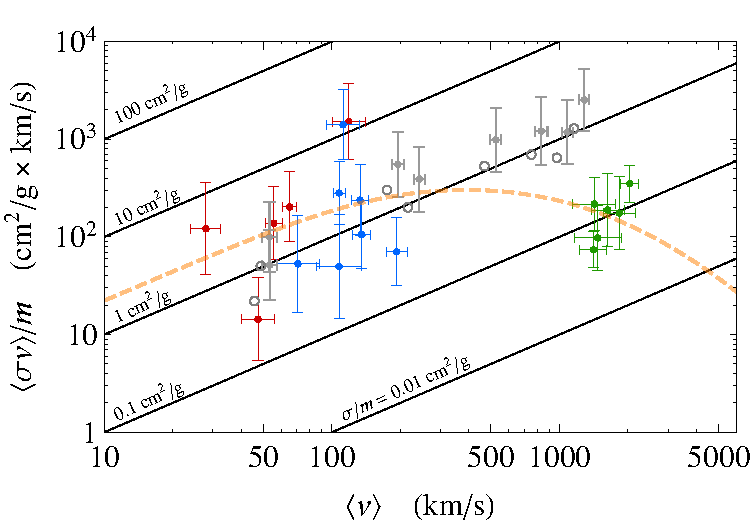
\includegraphics[width=0.6\columnwidth]{figures/sigmav.pdf}
\caption{Velocity-weighted self-interaction cross section per unit mass as a function of average relative particle velocity in a halo. Data points from astrophysical observations correspond to dwarf galaxies (red), low-surface-brightness galaxies (blue), and galaxy clusters (green). 
Diagonal lines show constant values of $\sigma/m_\chi$. 
Gray points are fits to mock data from SIDM simulations, with fixed $\sigma/m_\chi = 1 \cmg$.
Figure taken from \citet{Kaplinghat:2015aga}.
}
\label{fig:sidm_sigma}
\end{figure}

It is also natural to expect that SIDM has a modified matter power spectrum compared to CDM. For instance, in SIDM models where the dark matter particle couples to a massless particle in the early universe, either directly or through a light mediator, the tight coupling between dark matter and dark radiation can lead to dark acoustic oscillations \citep{Cyr-Racine:2013ab,Cyr-Racine:2013fsa}, resulting in a suppressed and oscillatory power spectrum \citep[\eg][]{1992ApJ...398...43C,Boehm:2001hm,Boehm:2004th,Feng:2009mn,Aarssen:2012fx}. It has been shown that realistic realizations of SIDM strongly prefer such a scenario \citep{ Huo:2017vef}.

To see the reach of LSST on the SIDM damping effect, we estimate the cut-off scale on the field halo mass due to the dark acoustic oscillations as $M_{\rm cut}\approx0.7\times10^{8}({\rm keV/T_{\rm kd}})^3 \Msun$~\citep{1512.05349}, where $T_{\rm kd}$ is the kinetic decoupling temperature. For SIDM models, where a dark matter particle ($\chi$) couples to a massless fermion ($f$) via a light mediator ($\phi$), $T_{\rm kd}$ is given by~\citep{Aarssen:2012fx,Cyr-Racine:2015ihg}
\begin{equation}
T_{\rm kd}\approx\frac{1.38~{\rm keV}}{\sqrt{g_\chi g_f}}\left(\frac{m_\chi}{100 \GeV}\right)^{\frac{1}{4}}\left(\frac{m_\phi}{10 \MeV}\right)\left(\frac{g_\star}{3.38}\right)^{\frac{1}{8}}\left(\frac{0.5}{\xi}\right)^{\frac{3}{2}},
\label{eq:tkd}
\end{equation}
where $g_f$ is the $\xi\textup{--}f$ coupling constant, $g_\star$ the is the number of massless degrees of freedom at decoupling and $\xi$ parameterizes the ratio of dark-to-visible temperatures. \citet{Huo:2017vef} recasts the Lyman-$\alpha$ bound on WDM to set upper limit on the decoupling temperature $T_{\rm kd}\gtrsim 1 \keV$, corresponding to the minimal halo mass $\roughly 10^8 \Msun$. Since LSST has the potential to extend measurements of the dark matter halo mass function by three orders of magnitude (\secref{halo_mass}), the expected sensitivity on the decoupling temperature is $T_{\rm kd}\sim 10 \keV$. If LSST detects a cutoff on the halo mass function, we can determine the corresponding $T_{\rm kd}$ and further narrow down the particle parameters contained in the Lagrangian via Eq.~(\ref{eq:tkd}) after combining with the measurements of $\sigma/m_\chi$ discussed above. Moreover, since the damping effect can also suppress the number of sub-halos in the Milky Way, we expect LSST to provide another constrain on $T_{\rm kd}$ in terms of the census of the ultra-faint satellites. In addition, although the acoustic damping effect may look similar to the free-streaming one \citep[\eg][]{1512.05349}, distinct signatures can be imprinted on the halo mass function \citep{Buckley:2014ab,Sameie:2018juk} or the Lyman-$\alpha$ forest spectrum \citep{Krall:2017xcw,Bose:2018juc}. By combining observables, including those from LSST, it might thus be possible to distinguish between WDM and SIDM with a damped matter power spectrum due to early-universe interactions (\secref{combine_probes}).

     
\subsection{Baryon-Scattering Dark Matter (BSDM) \Contact{Vera}}
\Contributors{Vera, Kim, ...}
\label{sec:bsdm}

In the standard WIMP scenario, dark matter may be directly observable through its scattering with Standard Model particles.
These models are conventionally probed by direct detection experiments that search for scattering between dark matter particles (from the local Galactic halo) and nuclei in their detectors.
These experiments are placed deep underground to provide shielding from cosmic-ray backgrounds and achieve exquisite sensitivity for low scattering cross sections. As a consequence of the depth of these experiments, the experiments have an upper bound to the cross section to which they are sensitive, because dark matter particles scatter many times in the Earth before reaching the experiment, losing most of their kinetic energy along the way \citep{Zaharijas:2004jv}.
%However, given the current null results from these experiments, 
Thus, it is important to broadly explore parameter space outside the standard WIMP region of interest.

Cosmological and astrophysical observables are unique and complementary probes of baryon-scattering dark matter (BSDM) models.
In particular, they are sensitive to very large (closer to nuclear-scale rather than weak-scale) scattering cross sections and sub-GeV dark matter masses, both of which are inaccessible to direct searches.
Such large cross sections may arise in a number of models.
One such model posits that dark matter is a flavor singlet sexaquark composed of $uuddss$ quarks \citep{Farrar:2017eqq}.
In this case, the scattering cross section with nucleons is expected to be geometric, though velocity-dependent enhancements may exist at very low energies, depending on the form of the sexaquark-nucleon potential.
For the sexaquark to be a viable dark matter candidate, it must be stable or have a sufficiently long lifetime; this criterion sets the sexaquark mass to be below a few GeV.
Alternatively, dark matter may be charged under a dark version of electromagnetism with field strength $\tilde{F}_{\mu\nu}$, which may kinetically mix with ordinary electromagnetism~\citep{Holdom:1985ag}:
\begin{equation}
    \mathcal{L} \supset \frac{\kappa}{2} F^{\mu\nu} \tilde{F}_{\mu\nu} ,
\end{equation}
where $\kappa$ parameterizes the strength of the mixing.
In this scenario, dark matter acquires a fractional amount of electric charge (proportional to $\kappa$ and its dark charge), allowing it to scatter with electrons and protons via Coulomb interactions that have a velocity dependence of $v^{-4}$.
This interaction is significant at late cosmological times, as the universe expands and the momentum of matter redshifts away.

Instead of focusing on particular theories, it is possible to describe the low-energy scattering processes of BSDM models with a nonrelativistic effective field theory~\citep{Fan:2010gt,Fitzpatrick:2012ix,Anand:2013yka}.
The effective Lagrangian has the form
\begin{equation}
    \mathcal{L}_\textrm{eff}(\vec{x})
    = c \Psi_\chi^\ast (\vec{x}) \mathcal{O}_\chi \Psi_\chi (\vec{x})
    \Psi_N^\ast (\vec{x}) \mathcal{O}_N \Psi_N (\vec{x}) ,
\end{equation}
where $\Psi (\vec{x})$ are the nonrelativistic fields for the dark matter, $\chi$, and nucleon, $N$.
Dark matter experiments seek to constrain and measure the coefficient $c$ for a variety of possible operators $\mathcal{O}_\chi$ and $\mathcal{O}_N$ that encode the BSDM physics.
However, regardless of the specific underlying BSDM model, cosmological observables are sensitive only to the magnitude (which scales as $c^2$) and velocity dependence of the cross section.
Thus, while laboratory searches for dark matter typically rely on assumptions about the detailed form of the interaction, cosmology offers very broad and generic probes of dark matter physics.

In a cosmological setting, scattering results in the exchange of momentum between the dark matter and the baryon fluids.
The momentum transfer induces a drag force, which suppresses structure increasingly at smaller scales. 
The effect of scattering is qualitatively similar to a cutoff in the matter power spectrum arising in the WDM and SIDM scenarios (\figref{dmbaryon_pk}).
This feature can be sought with tracers of matter on all observable scales. 
The best cosmological and astrophysical limits so far come from CMB temperature, polarization, and lensing anisotropy measurements~\citep{Xu:2018efh,Boddy:2018kfv,Gluscevic:2017ywp,Boddy:2018wzy,Slatyer:2018aqg}, cosmic-ray observations \citep{Cappiello:2018hsu}, and Lyman-$\alpha$-forest measurements~\citep{Dvorkin:2013cea,Xu:2018efh}. 
LSST will probe the matter power spectrum on even smaller scales, through substructure measurements from dwarf galaxies in the Local Volume, gaps in stellar streams, galaxy strong lensing, and galaxy-galaxy weak lensing; such observations will substantially extend sensitivity to BSDM models.  

\begin{figure}
\centering
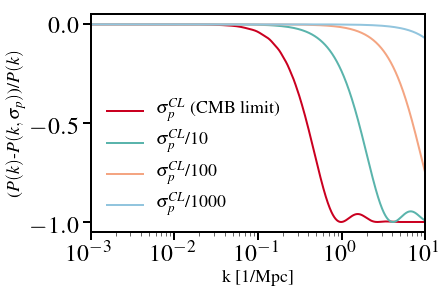
\includegraphics[width=0.6\columnwidth]{figures/dmbaryon_pk2.png}
\caption{Residuals in the linear matter power spectrum between the CDM case and a case where dark matter has a velocity-independent, spin-independent scattering with protons. The dark matter particle mass is set to $1\MeV$, and all other cosmological parameters are set to their best-fit Planck 2015 values \citep{Ade:2015xua}. Different residual curves display cutoffs at different angular scales, controlled by the magnitude of the interaction cross section. The highest cross section shown corresponds to the current 95\% confidence-level upper limit inferred from analyses of CMB data \citep{Gluscevic:2017ywp,Boddy:2018kfv}.
}
\label{fig:dmbaryon_pk}
\end{figure}

As an example, a measurement of the minimum halo mass translates into an upper limit on the dark matter-proton interaction cross section, based on the corresponding cutoff in the matter power spectrum $P(k)$. \figref{dmbaryon_pk} shows how the position of the cutoff in the linear $P(k)$ varies as a function of the interaction cross section. For example, a lower limit on the cutoff of $k_\text{cutoff} \sim 10/\Mpc$ roughly corresponds to an upper limit on the cross section which is 100 times more stringent than the current limit from CMB searches. Using limits on WDM as a proxy for a suppressed $P(k)$, a minimum halo mass of $\roughly 10^6 \Msun$ would imply an improvement of roughly five orders of magnitude compared to current best cosmological limits on the interaction cross section.

\section{Field Dark Matter \Contact{Chanda}}
\label{sec:axions}

While current observations of the matter power spectrum constrain the minimum mass of thermally produced dark matter, other mechanisms can  produce dark matter with significantly lower masses. The landscape of light dark matter candidates is vast, and in this section, we specifically focus on the class of axion-like particle (ALP) dark matter candidates.
ALP models span a wide range of viable parameter space (both in coupling strength and mass), and many of the observables described in this section can be generically applied to a broader class of light scalar particles.

The ALP paradigm was inspired by the QCD axion, which arises as a by-product of the most successful solution to the Strong CP Problem in the Standard Model \citep{PecceiQuinn:1977}. 
The cosmological abundance of axions is set by the Peccei-Quinn symmetry breaking scale, $f_\phi$, with a value
\begin{equation}
\Omega_\phi\sim\left(\frac{f_\phi}{10^{11-12}\,{\rm GeV}}\right)^{7/6}.
\end{equation}
This expression may be altered due to the temperature-dependence of the axion mass and ignorance about whether the Peccei-Quinn symmetry breaks before or after inflation. 
QCD theory gives no {\it a priori} prediction for the axion mass; however, in the context of dark matter composed of QCD axions, the axion mass is considered to be $m_\phi< 10^{-3}$ eV ($10^{-39}$ kg). 
If the initial misalignment angle is order unity, this yields a QCD axion mass of $m_\phi \sim 10^{-5}$ eV ($10^{-41}$ kg).
%\ADW{Please check Chanda!}
The broader category of ALPs possess QCD-axion-like potentials producing light scalar particles that obey a shift symmetry ($\phi \rightarrow \phi + 2\pi n$), but do not obey the same coupling between particle mass and symmetry breaking scale. 
ALPs can be motivated by string theory, where there are many moduli with axion-like potentials, and can produce a range of astrophysical phenomenology.
%ALPs can be sufficiently different from the QCD axion so as to produce notably different astrophysical phenomenology. 
ALPs may be non-thermally produced in the early universe and survive as a cold dark matter population until today \citep[\eg][]{Arias:2012az}.

%Fuzzy dark matter: In this scenario, dark matter is made of ultra light scalar particles with mass around $10^{-22}~{\rm eV}$. With such as a small mass, the de Broglie wavelength of the dark matter particle is $\mathcal{O}({\rm kpc})$, comparable to galaxy sizes, and the quantum effect becomes relevant in structure formation. Fuzzy dark matter predicts a solitonic core in the halo center and its size is set by the de Broglie wavelength of the dark matter particle. On larger scales, the structure predicted in fuzzy dark matter is less clumpy and less abundant than its CDM counterpart due to the quantum interference effect.

Astrophysical observations place the only known lower bound on the mass of ALPs and other non-thermally produced ultra-light particles, commonly described as ``fuzzy'' dark matter \citep[FDM; \eg,][]{Hu:2000,Hui:2017}. 
The de Broglie wavelength of these particles is constrained to be smaller than the size of the smallest galaxy, $\mathcal{O}(1\kpc)$, setting a lower limit on particle mass at $m_\phi \gtrsim 10^{-22}$ eV. 
%The formation of halos with mass $M_h \lesssim 10^{10} (m_\phi / 10^{-22} \eV)^{-4/3} \Msun$ will be significantly suppressed, and halos with $M_h \lesssim 10^7 (m_\phi / 10^{-22} \eV)^{-3/2} \Msun$ should not form at all \citep{Hui:2017}.
In addition, FDM is predicted to produce solitonic cores in the centers of halos, which would measurably effect the velocity profiles of dark-matter dominated galaxies \citep{Robles:2012uy,Robles:2018fur,Schive:2014hza,Du:2016aik}. 
On larger scales, the structure predicted in FDM is less abundant than its CDM counterpart due to quantum interference effects.
This is similar to the case of WDM, and again dark matter properties can be constrained through mesurements of the least massive dark matter halos.
Combining Equation 8 of \citet[][]{1703.09126} with \eqnref{Mhm} in \secref{wdm}, we can express constraints on the minimum FDM mass, $m_\phi$, as a function of the half-mode halo mass, $M_{\rm hm}$:
\begin{equation}
M_{\rm hm} = 1.2 \times 10^{11} \left( \frac{m_\phi}{10^{-22}\eV} \right)^{-1.4} \Msun,
\end{equation}
or expressed in terms of $m_\phi$, 
\begin{equation}
m_\phi = 3.1 \times 10^{-21} \left( \frac{M_{\rm hm}}{10^{9}\Msun} \right)^{-0.71} \eV.
\end{equation}
LSST will constrain the minumum mass of light bosonic dark matter to be greater than $m_\phi \sim 10^{-20} \eV$ by precisely constraing the half-mode mass to be less than $M_{\rm hm} \sim 10^{8} \Msun$.

%ADW: I think the paragraphs below have slightly too much much detail, for this report. It would be good to talk about axion stars, galaxy caustics, and anomalous energy loss in stellar populations and SN.
%CPW, 10/29/2018: I think some of it should be reintroduced, but I have shortened and edited to suggest these are different scenarios under consideration.
%Sikivie & Yang 2009

There has been significant debate in the literature about the astrophysical phenomenology of the QCD axion and ALPs.
\citet{Sikivie:2009} noted that because the axion is a scalar with high abundance in the early universe (circa matter-radiation equality), the axion could potentially settle into a Bose-Einstein condensate (BEC) state, whereby all particles can be described using one coherent ground state wave function. 
Furthermore, \citet{Sikivie:2009} argue that during the radiation-dominated era, axions will rethermalize into BECs with a Hubble-scale correlation length.
This could produce significant observational implications, such as several-kpc-scale caustic structures observable in the stellar distributions of the Milky Way and other low-redshift galaxies \citep[\eg,][]{Natarajan:2006,0805.4556,Rindler-Daller:2013zxa}.

On the other hand, \citet{1412.5930} argue that a particle such as the QCD axion, which has an attractive self-interaction, in an attractive gravitational potential will not sustain Hubble-scale correlations.
Instead, \citet{1412.5930} predict that axions will form coherent clumps that have been called ``Axion stars'' or ``Bose stars'' \citep[\eg][]{Kolb:1993}.\footnote{For the QCD axion it would be more appropriate to call these ``axteroids'' (a term coined by Anna Watts) due to their mass of $\roughly 10^{-11} \Msun$ \citep{Tkachev:1991ka,Braaten:2018nag}.} 
Looking beyond the QCD axion, for some ALP models, compact BEC ``miniclusters'' could form and grow to $\gtrsim 1\Msun$, at which point they may be detectable by LSST through mergers with other compact objects \citep{1808.04746} or through microlensing \citep{1707.03310}.

%What is distinct about this proposal is not so much the idea that the axion might begin as a BEC -- this seems likely (although making this statement formal is an open problem) -- but rather once the particles experience perturbations, do they remain in a BEC state? %These are distinct from the spherical topology predicted for WIMPs \citep{Bertschinger:2006nq}. 
%These massive compact structures could be detected through collisions with stellar remnants, which could be constrained by the transient event rate measured by LSST \citep{1808.04746}.
%Still other theories predict that axions could collapse 
%\ADW{I don't know if I believe either of these detection scenarios.}

%This proposal has a distinct phenomenology and LSST observations providing insights into caustics around nearby galaxies, may help distinguish between the two.

%Complicating LSST's capacity to distinguish between models is the possibility of degeneracy between the SY model and other axion-like particle phenomenologies. Both of the aforementioned scenarios, which have kicked off significant debate and renewed interest in Bose-Einstein condensed axion phenomenology, focus on the QCD axion in a mass range of around $10^{-5}$ eV. There is an extensive literature regarding axion phenomenology beyond the QCD axion and this mass range, e.g. ultralight axions (ULA) and fuzzy dark matter (FDM). In ULA/FDM scenarios, the De Broglie wavelength of the particle is such that the coherent wave can be halo-scale, which may give distinct stellar density distributions, which LSST will measure, than the SY proposal or the clump scenario.

Additional astrophysical constraints on ALPs generally come from proposed couplings with photons and/or electrons. 
For example, the Lagrangian can be expressed as,
\begin{equation}
    \mathcal{L} = -\frac{1}{2} \partial_\mu\phi\partial^\mu\phi + \frac{1}{2}m_\phi^2 \phi^2 - \frac{1}{4}g_{\phi\gamma}F_{\mu\nu}\tilde{F}^{\mu\nu}\phi - g_{\phi e}\frac{\partial_\mu\phi}{2m_e}\bar{\psi}_e \gamma^\mu\gamma_5\psi_e,
\end{equation}
where $g_{\phi\gamma}$ is the photon-axion coupling, $g_{\phi e}$ is the axion-electron coupling, $F^{\mu\nu}$ is the electromagnetic field tensor (and $\tilde{F}$ its dual), and $\psi_e$ is the electron field \citep[\eg][]{1302.6283,Redondo:2013wwa}.\footnote{Additional couplings to nucleons are allowed, but are not relevant for the LSST observations discussed here.}
For sufficiently large couplings to photons or electrons, the ALP can manifest as an additional anomalous energy loss mechanism, transporting energy out of the interiors of stars \citep[\eg,][]{Raffelt:1990}.
This energy loss could affect the evolution of stars, for example altering the lifetimes of giant stars \citep{Ayala:2014,Viaux:2013hca,Viaux:2013lha} or the cooling rate of white dwarf stars \citep{Isern:2008}.
The precise photometry of LSST will provide sensitive measurements of stellar populations to search for deviations from the predictions of standard stellar evolutionary models.

\begin{comment}
\TT{We should also mention the dark photon}
\ADW{Would we want to include some discussion of soliton cores from fuzzy DM?}

LSST will be able to probe axion dark matter in the following ways:
\begin{itemize}
    \item Caustics around Nearby Galaxies \CPW{11.25 Dealt with, now?}
    \item Anomalous Cooling in Stellar Populations 
    \begin{itemize}
        \item White dwarf luminosity function
        \item Globular cluster
        \item Cepheids / blue loop?
    \end{itemize}
    \item Supernova Observations
    
\end{itemize}
\end{comment}




\section{Compact Objects \Contact{Simeon}}
\label{sec:machos}
\Contributors{Simeon Bird, Juan Garc\'ia-Bellido, Will Dawson, Nathan Golovich, Michael Medford}
% George Chapline

Compact objects, particularly black holes formed in the early universe, represent one of the oldest and most venerable models of dark matter. Primordial black holes could originate from small-scale density fluctuations during the era of inflation. The same fluctuations that lay down the seeds of galaxies, if boosted on small scales, can lead to some small areas having a Schwarzschild mass within the horizon, which spontaneously collapse to form black holes. Because these black holes do not accrete or radiate strongly (at the time of formation there is no gas to form an accretion disc), they are a natural candidate for dark matter \citep{Carr:1974nx,Meszaros:1974,1975Natur.253..251C,Bellido:1996,Carr:2016drx}. 

Compact object dark matter is fundamentally different from particle models; primordial black holes cannot be studied in an accelerator and can only be detected through their gravitational force. Current constraints suggest that primordial black holes do not make up all of dark matter \citep[\eg][]{Sasaki:2018}. However, these constraints may be evaded if PBHs are spatially clustered \citep{Clesse:2015,Clesse:2017}. Moreover, primordial black holes are one possible source of the merging $30 \Msun$ black holes recently detected by LIGO \citep{Bird:2016,Clesse:2016}. This possibility has rekindled interest in these objects, both as a source of dark matter and in their own right.

Limits on the abundance and mass range of primordial black holes are wholly observational. The black hole mass is set by the mass enclosed within the horizon at the time of black hole collapse and thus ranges between $10^{-18} \Msun$ ($10^{15}\g$), below which the black hole would evaporate, and $10^9 \Msun$ ($10^{42}\g$), above which structure formation, Big Bang Nucleosynthesis and the formation of the microwave background would be severely affected \citep{Sasaki:2018}. 
For stellar mass black holes, the gold standard for detecting compact objects is microlensing. Current microlensing constraints set limits on the black hole abundance at the level of $10\%$ for black holes $0.01 - 10 \Msun$ \citep[however, see][]{2018MNRAS.479.2889C}. LSST will revolutionize the astrometric microlensing technique,  constraining the abundance of primordial black holes to a level of $10^{-4}$ of the dark matter over a wide range of masses (\secref{compact_objects}).

As primordial black holes form directly from the primordial density fluctuations, a measurement of their abundance would directly constrain the amplitude of density fluctuations \citep{Carr:1974nx, Meszaros:1974}. %1203.2681 
Although these constraints are several orders of magnitude weaker than, for example, those from the microwave background, they probe small scales between $k = 10^{7} - 10^{19}$ $h$/Mpc, much smaller than those measured by other current and future probes \citep{Bringmann:2012}. Because these scales are highly non-linear in the late-time universe, there is no other possible constraint; the information present at early times has been washed away by gravitational evolution. Primordial black holes are thus a probe of primordial density fluctuations in a range that is inaccessible to other techniques~\citep{Josan:2009,Bellido:2017,Bellido:2018}. These curvature fluctuations are imprinted on space-time hypersurfaces during inflation, at extremely high energies, beyond those currently accessible by terrestrial and cosmic accelerators. 
Our understanding of the universe at these high energies, of order $10^{15} \GeV$ and above, comes predominantly from extrapolations of known physics at the electroweak scale.
%At these high energies, of order $10^{15} \GeV$ and above, there are few theoretical constraints, and most of our assumptions come from extrapolations of known physics at the electroweak scale. 
Measurements of the primordial density fluctuations via the abundance of primordial black holes would provide unique insights into physics at these ultra-high energies.

%For example, the long lever of scales means that the constraints on simple scale-invariant inflation models expressed in terms of a scalar index, $n_s$ and a running, $\alpha_s$ can be competitive for some models. 

Furthermore, it may be possible for LSST to constrain the existence of ultra-compact mini-halos using correlated microlensing signals \citep{erickcek2011,li2012}. These objects arise from initial overdensities that are too small to collapse into primordial black holes. These overdensities still collapse at high redshift to form low-mass halos; thus, since these objects form early and have few mergers \citep{Bringmann:2012,Delos:2018}, they have a high concentration and a steeper internal density profile than the standard Navarro-Frenk-White shape. In turn, this makes them easier to detect via lensing and harder to disrupt than standard CDM subhalos. Current constraints on these objects are highly model-dependent. In particular, they largely come from counting gamma-ray photons from astrophysical sources under the assumption of a WIMP dark matter annihilation cross-section. LSST will place new constraints on the existence of small halos via micro-lensing and thereby constrain the physics of the inflaton on scales of $k = 10 \textup{--} 10^7 h$/Mpc for the first time in a model-independent way.

%See Figure 6 of Bringmann 2012: \url{https://arxiv.org/abs/1110.2484}
%Sasaki 2018: \url{https://arxiv.org/abs/1801.05235}

